\chapter{Implementation and experimental results} \label{chap:experimental_results}

In Chapter \ref{chap:methods} and \ref{chap:independent_set} we discussed different heuristics aimed at solving the the matrix partitioning problem; whether we try to improve the initial partitioning or perform a fully iterative procedure, we need to translate those ideas into practice, devising an efficient implementation.

In Section \ref{sec:earlier_work}, we mentioned existing software partitioners: Mondriaan \cite{mondriaan} is the package of our choice and we defer to it the actual computations of the partitionings, limiting ourselves to create the matrix $B$ of the medium-grain model as in \eqref{eq:Bmatrix}. The actual algorithm used to construct this matrix is given explicitly in Algorithm \ref{alg:B}. Note how we consider only the sparsity patterns of $A$, neglecting completely the values of the nonzeros.

\begin{algorithm}[h]
	\begin{algorithmic}
		\Require{$A_r$, $A_c$}
		\Ensure{$B$}
		\State $B \gets \varnothing$
		\ForAll{$a_{ij} \in A_c$} \Comment{The part relative to $A_c$}
		\State $b_{i+n,j} = 1$
		\EndFor
		\ForAll{$a_{ij} \in A_r$} \Comment{The part relative to $A_r$}
		\State $b_{j,i+n} = 1$
		\EndFor
		\For{$j=1,\dots,n$} \Comment{Dummy nonzeros for cut columns}
		\If{$\exists\, i$ s.t. $a_{ij} \in A_r$ and $\exists\, i'$ s.t. $a_{i'j} \in A_c$}
		\State $b_{j,j} = 1$
		\EndIf
		\EndFor
		\For{$i=1,\dots,m$} \Comment{Dummy nonzeros for cut rows}
		\If{$\exists\, j$ s.t. $a_{ij} \in A_r$ and $\exists\, j'$ s.t. $a_{ij'} \in A_c$}
		\State $b_{n+i,n+i} = 1$
		\EndIf
		\EndFor
	\end{algorithmic}
	\caption{Construction of $B$ following the medium-grain model.} \label{alg:B}
\end{algorithm}

Now, having discussed the means of obtaining $A_r$ and $A_c$ and the matrix $B$, we can outline the general framework used to test the effectiveness of the proposed heuristics. The framework is given explicitly in Algorithm \ref{alg:framework}, and it takes as a parameter the maximum number of iterations allowed, $iter_{max}$.  

\begin{algorithm}[h]
	\begin{algorithmic}
		\Require{Sparse matrix $A$}
		\Ensure{Partitioning for the matrix $A$}
		\State Partition $A$ with Mondriaan using the default options and the medium-grain method
		\For{$i=1,\dots,iter_{max}$}
		\State Use any of the heuristics described previously to compute $A_r$ and $A_c$
		\State construct $B$, using Algorithm \ref{alg:B}, from $A_r$ and $A_c$
		\State Partition $B$ with Mondriaan using the default options and the row-net model
		\State Re-construct $A$ with the new partitioning
		\EndFor
	\end{algorithmic}
	\caption{General framework for the testing of our heuristics} \label{alg:framework}
\end{algorithm}

In Chapter \ref{chap:methods} and \ref{chap:independent_set}, we distinguished between partition-oblivious and partition-aware methods, and Algorithm \ref{alg:framework} is suitable for both types of heuristics: even though the framework is naturally suited for developing a fully iterative scheme, if we desire a better initial partitioning for the medium-grain method, we can simply neglect the partitioning done in the first step. This is precisely the scope of a partition-oblivious heuristic.

Regarding the actual implementation, we can see from Algorithm \ref{alg:framework} that Mondriaan is used to perform the actual partitioning and this is the ideal case for its use as a software library. As a consequence, we used C as the main implementation language, even though MATLAB was used for faster prototyping: the flexibility added by managing objects at runtime  is ideal when designing algorithms. In order to have C code and MATLAB code interact in the correct way, we took advantage of MEX files \cite{mex}. In general, unless preliminary tests showed that the considered heuristic had a remarkably bad quality, we translated back most of the programs to the C language, in order to remove the MEX layer of complexity and get a more efficient implementation. For the Hopcroft-Karp algorithm described in Chapter \ref{chap:independent_set}, we used an implementation \cite{hkarp_impl} written in the Python programming language, which computes directly the matching on a bipartite graph and the maximum independent set. 

In order to perform effective numerical experiments, we need to have a consistent way of testing. First of all, since we seek heuristics suitable for many matrices, it makes sense to have several matrices to test for, as described in Section \ref{sec:test_matrices}. 

Secondly, since randomness is involved in the partitioner itself and, to a different extent, in some of the heuristics, need to perform several measurements and compute an average. After generating an initial partitioning, one iteration of the heuristic was performed independently 5 times, and their result was averaged; this was repeated 20 times, obtaining an average of the 20 initial partitioning and an average of the 20 averages of final results. 

Lastly, in order to have a meaningful result that can help us understand whether the given heuristic is globally effective, we will compute the geometric mean of all the initial partitioning and the geometric mean of all the final results. Then, we will normalize w.r.t the first value. Doing so, we can understand whether the considered heuristic performs better or worse in a consistent way. This normalized geometric mean is denoted, in the following tables, with the symbol $\rho$.

\section{Test matrices} \label{sec:test_matrices}

In order to have insightful results, we mentioned that the matrices used in the numerical experiments should have different features: in particular we distinguish between (strongly) rectangular matrices and square matrices, and try to have a wide selection w.r.t. the number of nonzeros. 

These matrices are mainly from the University of Florida Sparse Matrix Collection \cite{ufl}, and some can additionally be found on the Matrix Market collection \cite{matrixmarket}. The matrices \verb|tbdmatlab| and \verb|tbdlinux| are from \cite{mondriaan}. Table \ref{tab:matrices} provides a more thorough description of the matrices used, along with an outline of their basic properties (number of rows $m$, number of columns $n$, number of nonzeros $N$) and their original purpose. Some of these matrices (namely the ones with the $\dagger$ symbol in the table) belong to the 10th Dimacs Implementation Challenge \cite{dimacs}, which addressed the graph partitioning and graph clustering problem, and are therefore naturally suited for testing the quality of the solutions produced by our algorithms. The three symmetric matrices which represent street networks, are the undirected and unweighted version of the largest strongly connected component of the corresponding OpenStreetMap road network.

\begin{table}[h]
	\centering
	\begin{tabular}{|l|r|r|r|p{7cm} |}
		\hline	
		\textbf{Name} & \textbf{$m$} & \textbf{$n$} & \textbf{$N$} & \textbf{Source problem} \\ \hline
		\verb|lpi_ceria3d| 									& 3576 		& 4400 		& 21178 & Netlib Linear Programming \\
		\verb|dfl001| 											& 12230 	& 6071 		& 35632 & Netlib Linear Programming \\ 
		\verb|delaunay_n15| $\dagger$ 			& 32768 	& 32768 	& 196548 & Delaunay triangulations of random points in plane \\ 
		\verb|deltaX| 											& 68600 	& 21961 	& 247424 & High fillin with exact partial pivoting \\
		\verb|cre_b| 												& 9648 		& 77137 	& 260785 & Netlib Linear Programming \\ 
		\verb|tbdmatlab| 										& 19859 	& 5979 		& 430171 & Term-by-document matrix \\ 
		\verb|nug30|												& 52260 	& 379350 	& 1567800 & Netlib Linear Programming \\ 
		\verb|coAuthorsCiteseer| $\dagger$ 	& 227320 	& 227320 	& 1628268 & Citation and coauthor network\\ 
		\verb|bcsstk32| $\dagger$ 					& 44609 	& 44609 	& 2014701 & Stiffness matrix for automobile chassis \\ 
		\verb|bcsstk30| $\dagger$						& 28924 	& 28924 	& 2043492 & Stiffness matrix for off-shore generator platform \\
		\verb|wave| 	$\dagger$							& 156317 	& 156317 	& 2118662 & 3D finite elements \\
		\verb|tbdlinux| 										& 112757 	& 20167 	& 2157675 & Term-by-document matrix \\
		\verb|rgg_n_2_18_s0| $\dagger$ 			& 262144 	& 262144 	& 3094566 & Random graph \\
		\verb|belgium_osm| $\dagger$				& 1441295 & 1441295 & 3099940 & Street network of Belgium\\
		\verb|polyDFT| 											& 46176 	& 46176 	& 3690048 & Polymer self-assembly \\ 
		\verb|netherlands_osm| $\dagger$		& 2216688 & 2216688 & 4882476 & Street network of The Netherlands \\
		\verb|cage13| 											& 445315 	& 445315 	& 7479343 & DNA Electrophoresis \\
		\verb|italy_osm| $\dagger$					& 6686493 & 6686493 & 14027956 & Street network of Italy\\
		\hline
	\end{tabular}
	\caption{Matrices used in our experiments, sorted by number of nonzeros.} \label{tab:matrices}
\end{table}

In Figures \ref{fig:patterns1}, \ref{fig:patterns2} and \ref{fig:patterns3}, we show the sparsity patterns of the test matrices. The images were obtained using the \verb|spy| function of MATLAB.

%\begin{figure}[h]
%	\centering
%	\subfigure[\texttt{lpi\_ceria3d}]{ 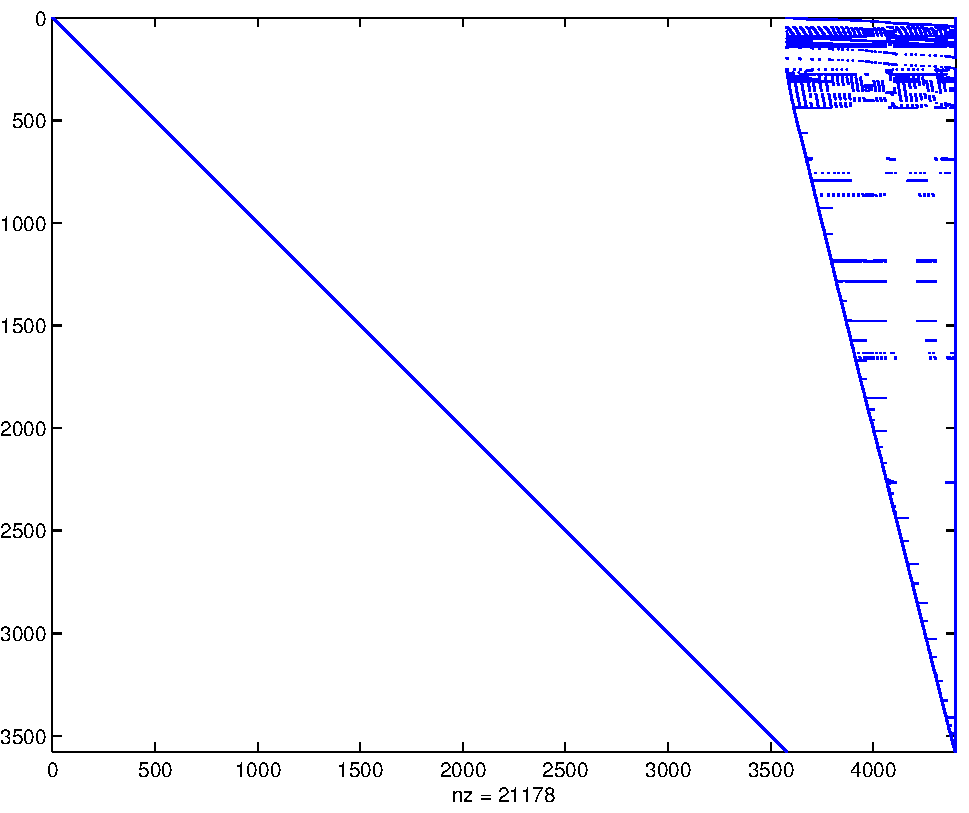
\includegraphics[scale=0.45]{img/lpi_ceria3d.pdf} \label{fig:lpi_ceria3d}}
%	\subfigure[\texttt{dfl001}]{ 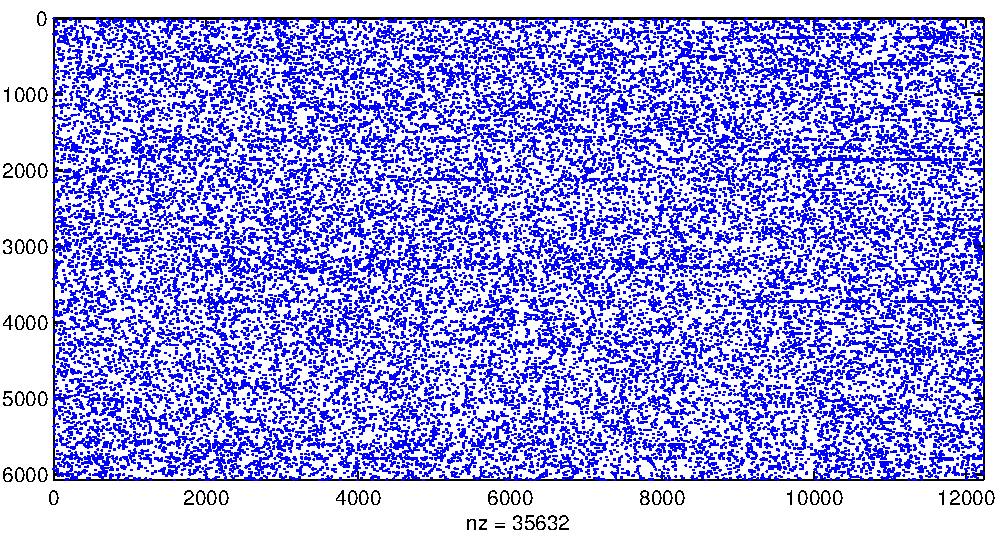
\includegraphics[scale=0.45]{img/dfl001.pdf} }
%	
%	\subfigure[\texttt{delaunay\_n15}]{ 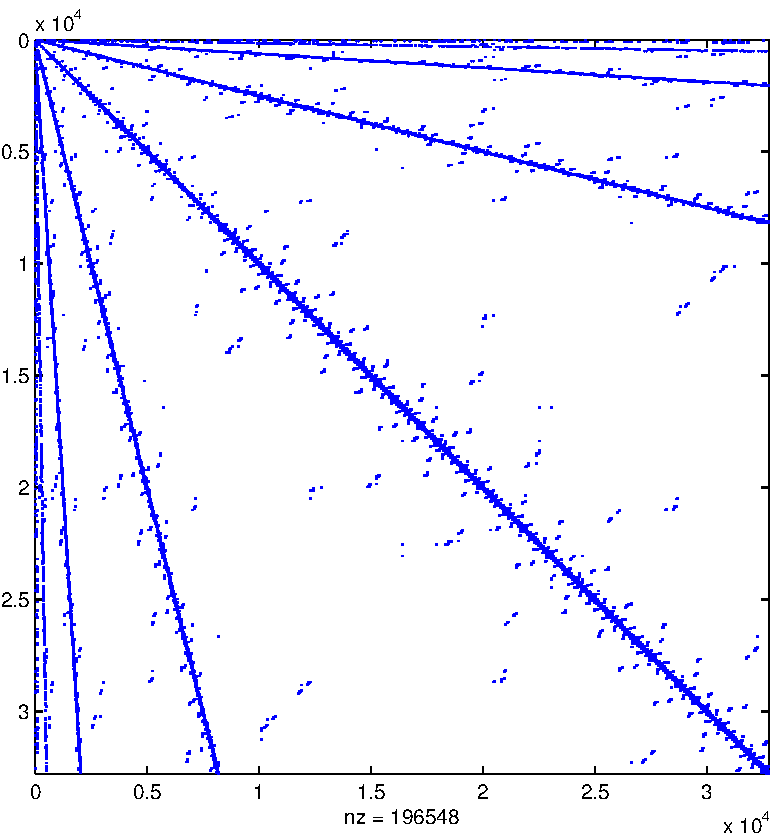
\includegraphics[scale=0.45]{img/delaunay_n15.pdf} }
%	\subfigure[\texttt{deltaX}]{ 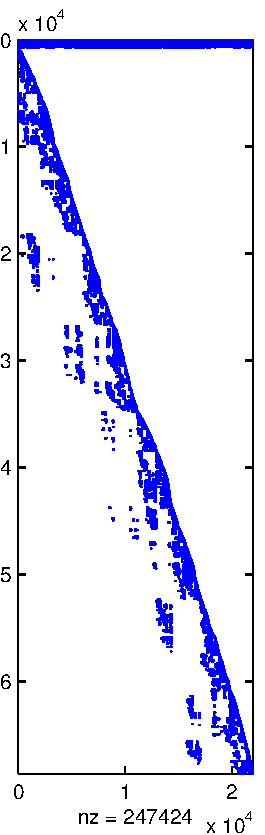
\includegraphics[scale=0.45]{img/deltaX.pdf} }
%	
%	\subfigure[\texttt{cre\_b}]{ 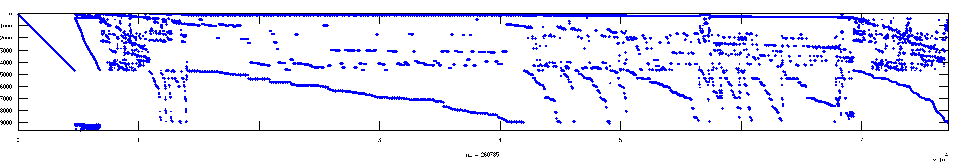
\includegraphics[scale=0.45]{img/cre_b.pdf} }
%	\subfigure[\texttt{tbdmatlab}]{ 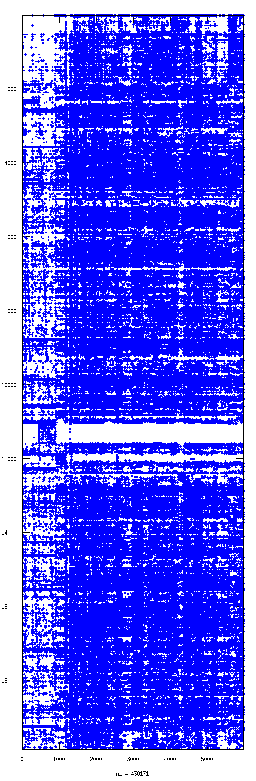
\includegraphics[scale=0.45]{img/tbdmatlab.pdf} }
%	\caption{Sparsity patterns of the test matrices.} \label{fig:patterns1}
%\end{figure}
%
%\begin{figure}[h]
%	\centering
%	\subfigure[\texttt{nug30}]{ 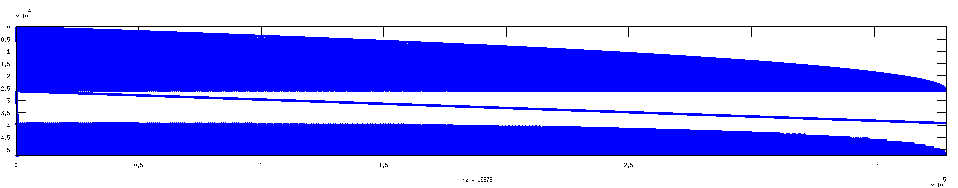
\includegraphics[scale=0.45]{img/nug30.pdf} }
%	\subfigure[\texttt{coAuthorsCiteseer}]{ 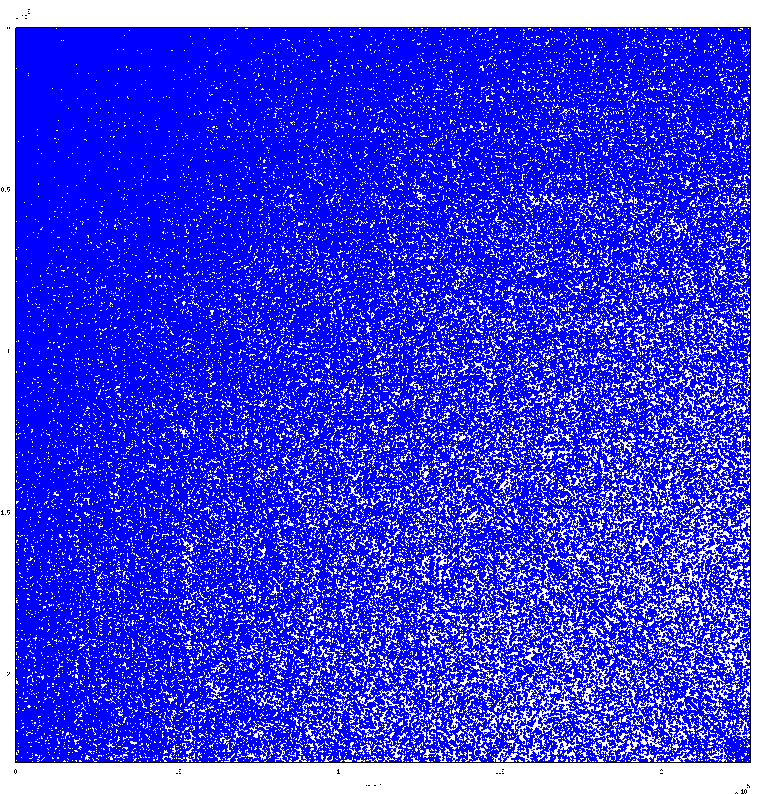
\includegraphics[scale=0.45]{img/coAuthorsCiteseer.pdf} }
%
%	\subfigure[\texttt{bcsstk30}]{ 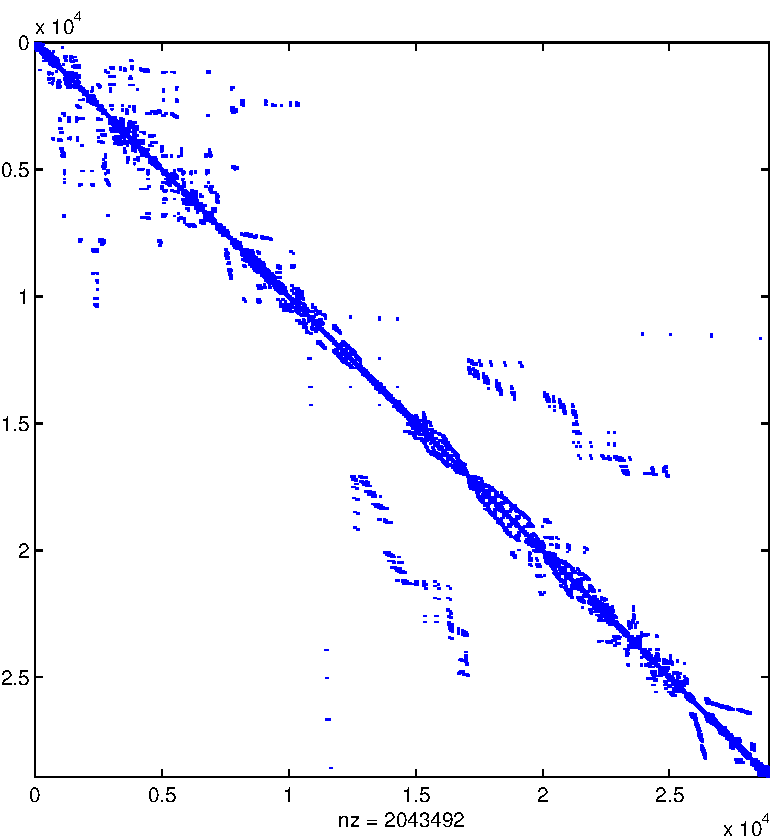
\includegraphics[scale=0.45]{img/bcsstk30.pdf} }
%	\subfigure[\texttt{bcsstk32}]{ 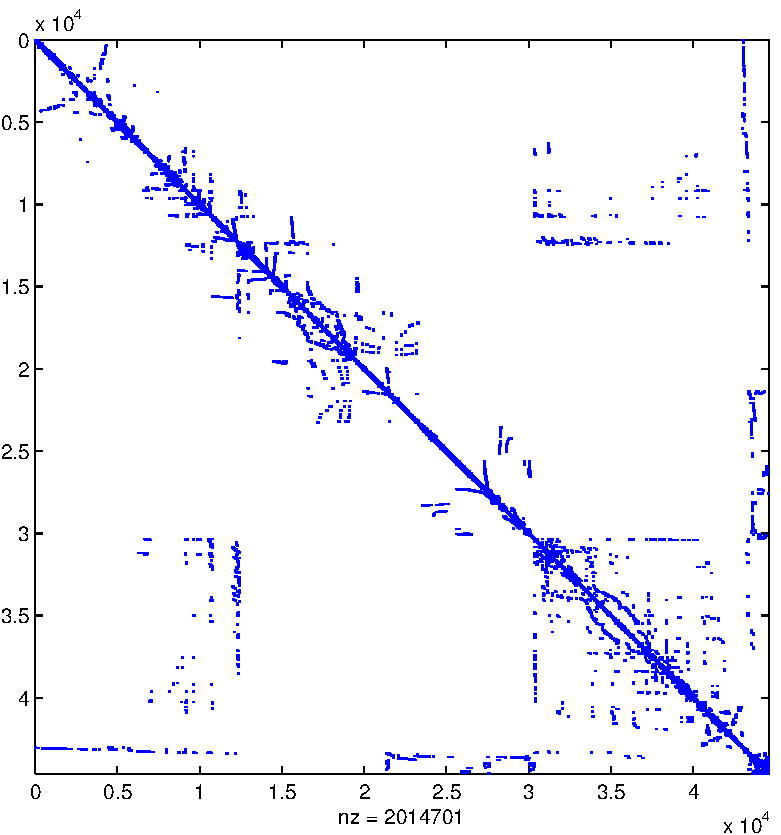
\includegraphics[scale=0.45]{img/bcsstk32.pdf} }
%	
%	\subfigure[\texttt{wave}]{ 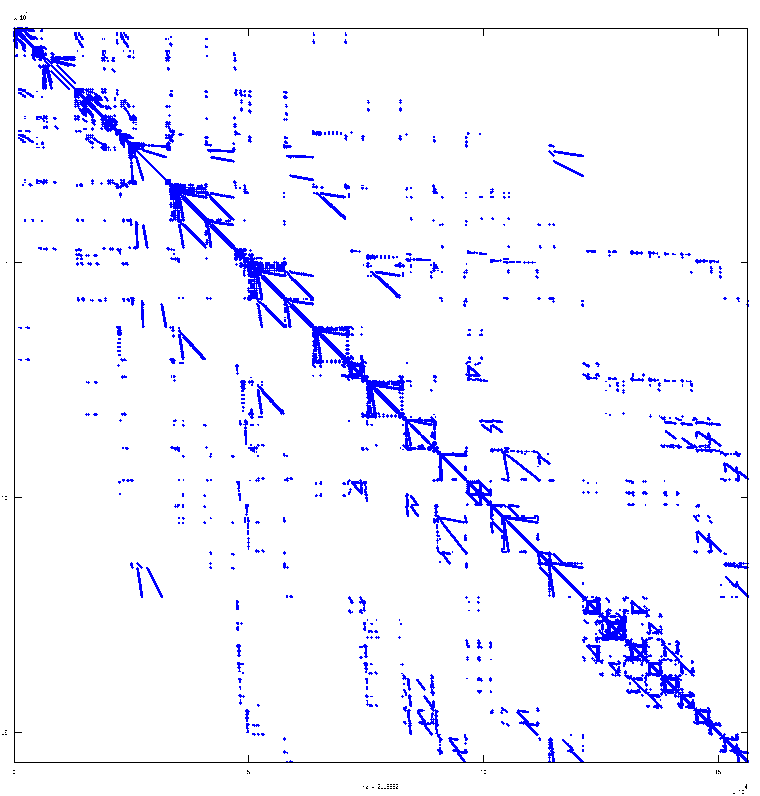
\includegraphics[scale=0.45]{img/wave.pdf} }
%	\subfigure[\texttt{tbdlinux}]{ 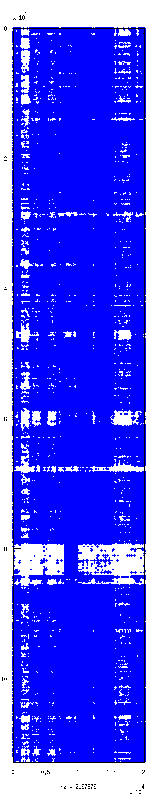
\includegraphics[scale=0.45]{img/tbdlinux.pdf} }
%	\caption{Sparsity patterns of the test matrices.} \label{fig:patterns2}
%\end{figure}
%
%\begin{figure}[h]
%	\centering
%	\subfigure[\texttt{rgg\_n\_2\_18\_s0}]{ 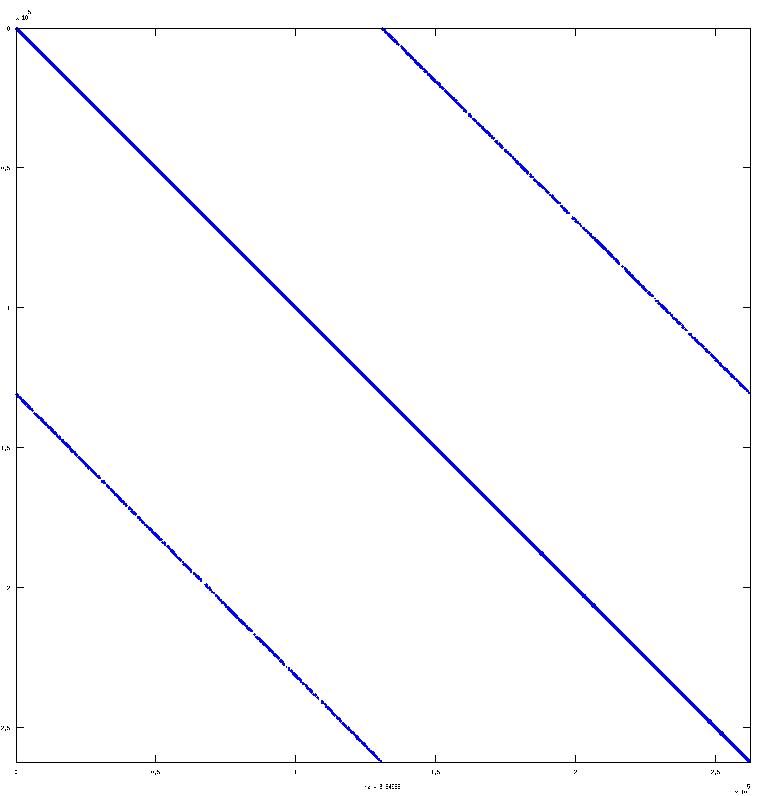
\includegraphics[scale=0.45]{img/rgg_n_2_18_s0.pdf} }
%	\subfigure[\texttt{belgium\_osm}]{ 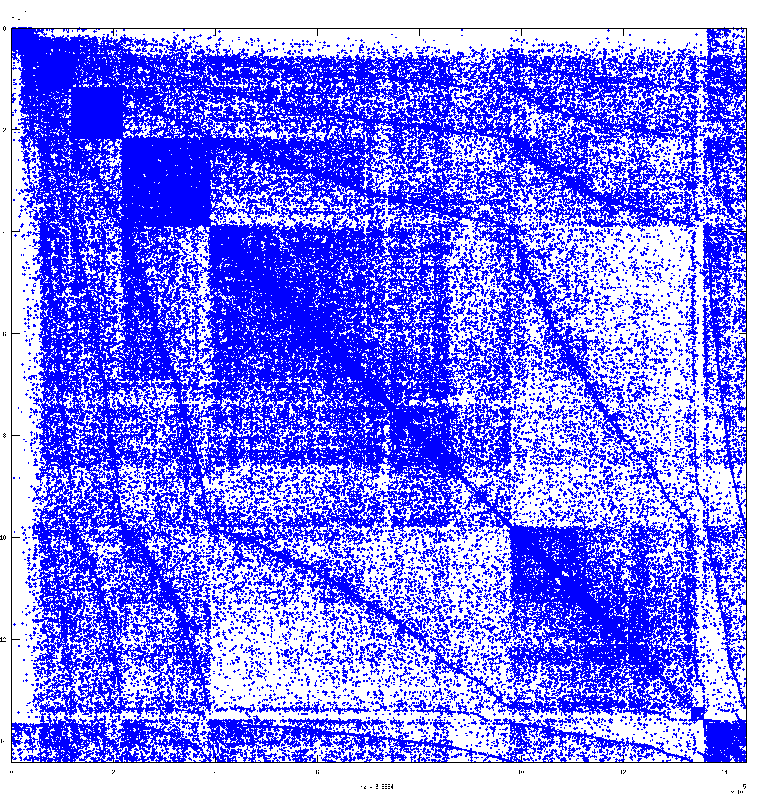
\includegraphics[scale=0.45]{img/belgium_osm.pdf} }
%	
%	\subfigure[\texttt{polyDFT}]{ 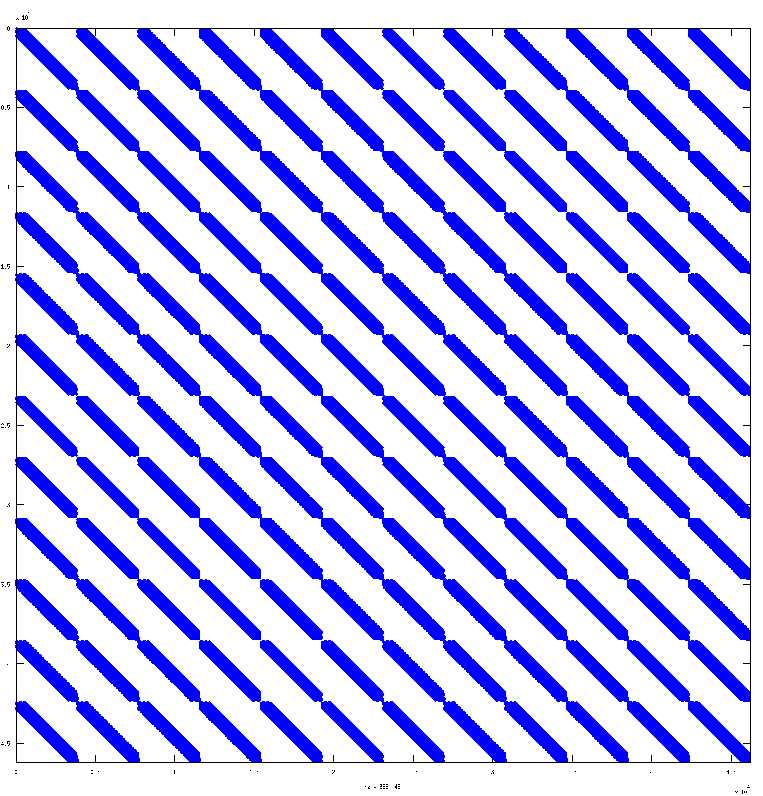
\includegraphics[scale=0.45]{img/polyDFT.pdf} }
%	\subfigure[\texttt{netherlands\_osm}]{ 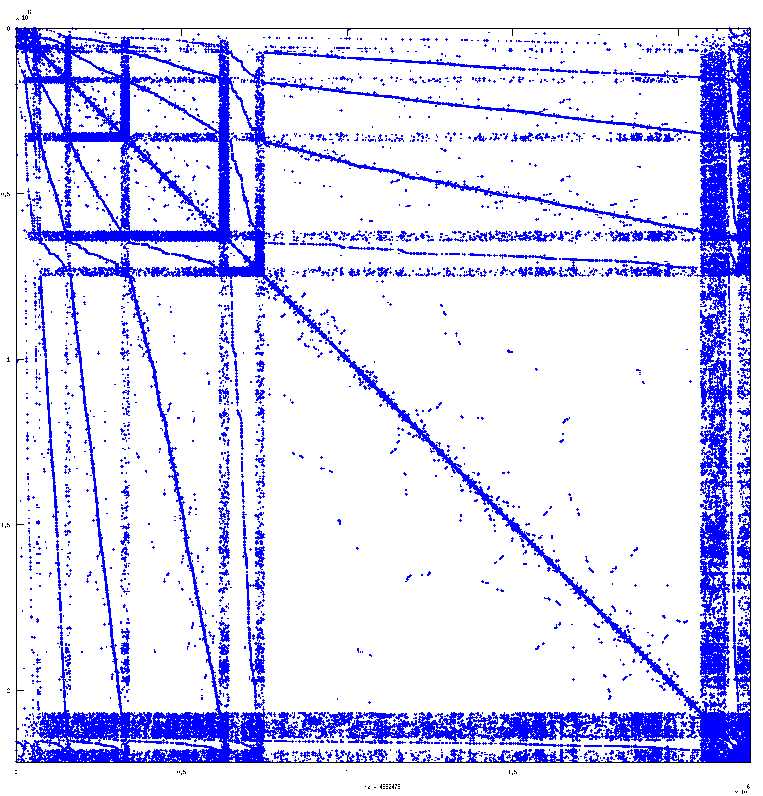
\includegraphics[scale=0.45]{img/netherlands_osm.pdf} }
%	
%	\subfigure[\texttt{cage13}]{ 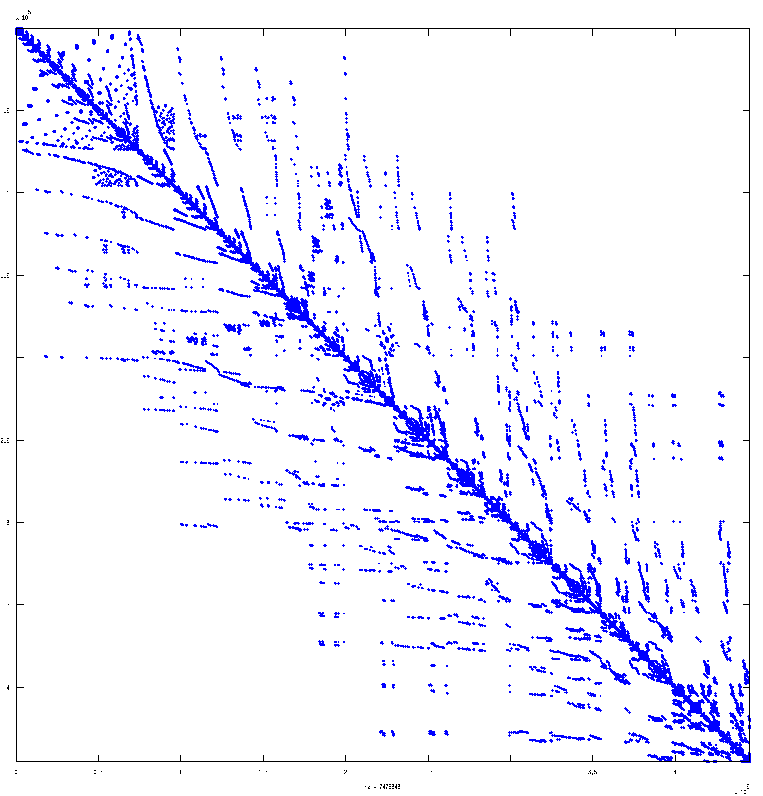
\includegraphics[scale=0.45]{img/cage13.pdf} }
%	\subfigure[\texttt{italy\_osm}]{ 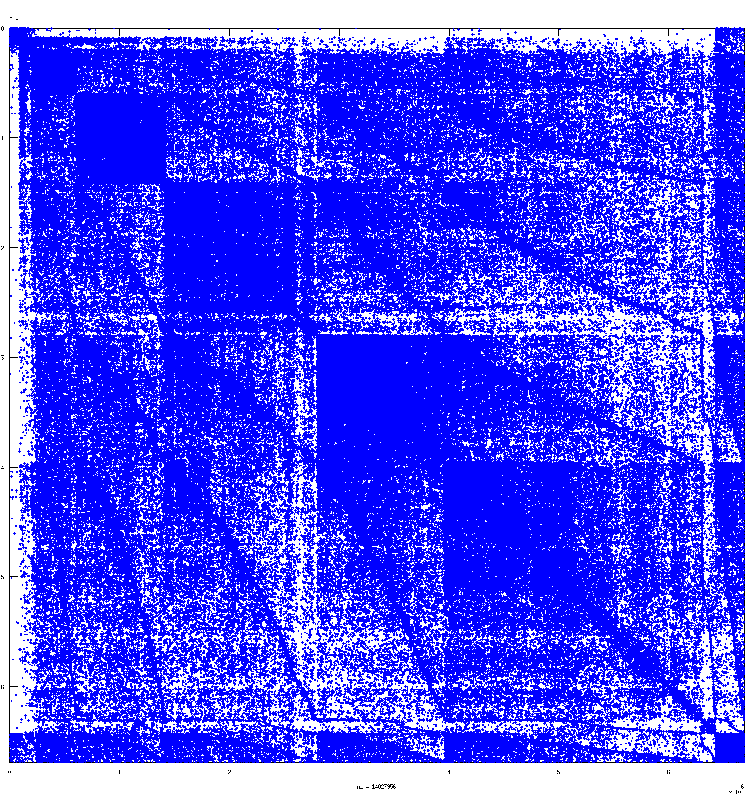
\includegraphics[scale=0.45]{img/italy_osm.pdf} }
%	\caption{Sparsity patterns of the test matrices.} \label{fig:patterns3}
%\end{figure}

\section{Preliminary selection of the best heuristics} \label{sec:preliminary_tests}

In Chapter \ref{chap:methods} and \ref{chap:independent_set} we discussed many heuristics, which in turn depend on different parameters. It is best to perform a preliminary analysis to quickly figure out which produce the best solutions and should therefore be tested extensively, and the ones that should not be further considered.

For this reason, a small number of different matrices (with a relatively small number of nonzeros) has been selected from our choice of Table \ref{tab:matrices}: in particular the considered matrices, which have a different structure, are \verb|dfl001|, \verb|tbdlinux|, \verb|nug30|, \verb|rgg_n_2_18_s0|, \verb|bcsstk30|.

The local search heuristic given in Section \ref{sec:globalview}, quickly turned out to be far from effective, and therefore we decided to discard it altogether in the numerical experiments.

In the following tests, the parameter $iter_{max}$ has been set to 1, which means that we are only perfoming one iteration of our heuristic. The reason for this choice will become clear in Section \ref{sec:iter_max}; for now, we will just take advantage of the fact that performing only one iteration is relatively fast and we can quickly get an idea about the best heuristics.

\subsection{Partition-oblivious heuristics} \label{sec:preliminary_po}

Table \ref{tab:preliminary_po} summarizes the results of this preliminary analysis of the partition-oblivious heuristics for the 5 chosen matrices. In the first line, the results of the medium-grain with the algorithm proposed in \cite{mediumgrain} are given. The value $\rho$ represents the geometric mean of the results for a given heuristic, averaged over all matrices and normalized w.r.t. the default medium-grain method.

\begin{table}[h]
	\centering

	\renewcommand{\arraystretch}{1.2}
	\begin{tabular}{|l||c|c|c|c|c||c|}
		\hline
		\multirow{2}{*}{\textbf{Heuristic}} &  \multicolumn{5}{|c||}{\textbf{Matrix}} & \multirow{2}{*}{$\rho$} \\ \cline{2-6}
		& \texttt{dfl001} & \texttt{nug30} & \texttt{bcsstk30} & \texttt{tbdlinux} & \texttt{rgg\_n\_2\_18\_s0} & \\ \hline
		medium-grain & 590 & 36262 & 552 & 8135 & 910 & 1.0 \\ \hline %2445
		\verb|po_localview|& \textbf{571} & 36665 & \textbf{598} & 8327 & 1160  & 1.07 \\  %2609.2
		\verb|po_unsorted_concat_row|& 1492 & 189689 & 653 & 15081 & 1098 & 2.04 \\ % 0 0 0 %4979.1
		\verb|po_unsorted_concat_col|& 589 & 38491  & 600 & 24024 & \textbf{1066} & 1.32 \\ % 0 1 0 %3224.1
		\verb|po_unsorted_random|& 1314 & 113070 & 1127 & 20154 & 1093 & 2.11 \\  % 2 0 0 %5169
		\verb|po_unsorted_mix_alt|& 1461 & 181216 & 715 & 27942 & 1104 & 2.32 \\  % 4 0 0 % 5666
		\verb|po_unsorted_mix_spr|& 1322 & 81915 & 759 & 18584 & 1122 & 1.81 \\  % 4 1 0 % 4434
		\verb|po_sorted_w_simple|& 597 & 38383 & 785  & 8307 & 1093 & 1.13 \\ % 6 0 0 % 2771
		\verb|po_sorted_nw_simple|& 606 & 38674 & 789 & \textbf{8301} & 1096 & 1.14 \\ % 6 1 0 % 2787
		\verb|po_sorted_w_concat_row|& 1486 & 189681 & 642 & 15082 & 1078 & 2.01 \\ % 8 1 0 % 4907
		\verb|po_sorted_w_concat_col|& 597 & 38655 & 621 & 24045 & 1068 & 1.33 \\  % 8 1 1 % 3261
		\verb|po_sorted_nw_concat_row|& 1496 & 189683 & 614 & 15086 & 1090 & 2.01 \\ % 8 0 0 % 4913
		\verb|po_sorted_nw_concat_col|& 593 & 38513 & 621 & 24005 & 1076 & 1.33 \\ % 8 0 1 % 3256
		\verb|po_sorted_w_mix_alt|& 1317 & 162549 & 790 & 23683 & 1091 & 2.19 \\ % 10 0 1 % 5346
		\verb|po_sorted_w_mix_spr|& 641 & 163013 & 782 & 23441 & 1093 & 1.88 \\ % 10 0 0 % 4615
		\verb|po_sorted_nw_mix_alt|& 1457 & 62273 & 797 & 15015 & 1096 & 1.69 \\ % 10 1 0  % 4122
		\verb|po_sorted_nw_mix_spr|& 719 & 62402 & 793 & 15072 & 1106 & 1.47 \\  % 10 1 1 % 3586
		\verb|po_is|& 594 & \textbf{30655} & 615 & 13286 & -  & 1.12 \\ % 3491 
		\hline
	\end{tabular}
	\caption{Results of the devised partition-oblivious heuristics for the five chosen matrices. In each column, we use boldface to highlight the best found partitioning (not considering the medium-grain value).} \label{tab:preliminary_po}
\end{table}

In the table there is no result for the heuristic \verb|po_is| and the  matrix \verb|rgg_n_2_18_s0|, because the maximum number of levels of recursion was reached before the algorithm completed.


The first method shown in the table, discussed in Section \ref{sec:localview}, shows the best results among these partition-oblivious heuristics. This is not surprising, as such algorithm is quite similar to the one originally proposed in \cite{mediumgrain}; \verb|po_localview| performs slightly worse (7\%, on average) than \verb|medium-grain| because the latter also includes an iterative refinement procedure \cite[Section 3.3]{mediumgrain}: after the partitioning is performed, the matrix $B$ is constructed by assigning all the nonzeros that belong to processor 0 to $A_r$ and the ones that belong to processor 1 to $A_c$, then the corresponding hypergraph is created and a single run of the Kernighan-Lin heuristic is performed; this procedure (which does not increase the communication value) is repeated until there are no more improvements, then the roles of $A_r$ and $A_c$ are inverted and the procedure is restarted. This fairly cheap scheme, computationally speaking, is repeated several times, until no further reduction can be obtained. 

From the table, it appears that the framework discussed in Section \ref{sec:hot_restart} is not particularly effective in this case: some methods result even in twice the communication volume, on average; the \verb|po_sorted_w_simple| and \verb|po_sorted_nw_simple| heuristics produce the best results with a communication volume, respectively, 13\% and 14\% worse than the reference value. Moreover, it appears that mixing rows and columns in the priority vector is not advisable: for the matrices \verb|dfl001| and \verb|ug_30|, for example, we obtain a communication volume 3-5 times higher than \verb|medium-grain|. 

The heuristic that employs the computation of the maximum independent set on the full matrix produces interesting results, especially with the matrix \verb|nug30|: the communication volume is, on average, 16\% lower than the one obtained with the medium-grain method; with the other matrices (in particular \verb|tbdlinux|), however, the results are not as satisfactory.

From this preliminary testing, we should choose the heuristic \verb|po_localview| and \verb|po_is| for further testing in Section \ref{sec:final_tests}

\subsection{Partition-aware heuristics} \label{sec:preliminary_pa}

In Table \ref{tab:preliminary_pa}, we summarize the results for the partition-aware heuristics. As now we are considering a fully iterative framework, it is best to explicitly give the average of the 20 initial partitionings (iteration 0) alongside the average of the 20 final results (iteration 1). The value $\rho$ represents, similarly as before, the geometric mean of the final results, normalized w.r.t. the average of the initial partitionings. 

\begin{table}[h]
	\centering
	\renewcommand{\arraystretch}{1.15}
	\begin{tabular}{|l|c||c|c|c|c|c||c|}
		\hline
		\multirow{2}{*}{\textbf{Heuristic}} & \multirow{2}{*}{$i$} &  \multicolumn{5}{|c||}{\textbf{Matrix}} & \multirow{2}{*}{$\rho$} \\ \cline{3-7}
		& & \texttt{dfl001} & \texttt{nug30} & \texttt{bcsstk30} & \texttt{tbdlinux} & \texttt{rgg\_n\_2\_18\_s0} & \\ \hline
		\verb|pa_localview| & 0 & 582 & 36224 & 537 & 8051 & 914 &   \\ % 2422
		& 1 & \textbf{575} & 36896 & 577 & 9934 & 2189 & 1.26 \\ \hline %3055

		\verb|pa_sbdview| & 0 & 590 & 36057 & 546 & 8112 & 899 & \\ % 2430
		& 1 & 1493 & 187241 & 699 & 19852 & 1074 & 2.17 \\ \hline % 5296

		\verb|pa_sbd2view| & 0 & 583 &  36123 & 542 & 8018 & 906 &  \\ % 2419
		& 1 & 1276 & 125009 & 1150 & 20757 & 1055 & 2.17 \\ \hline % 5258
		
		\verb|pa_unsorted_concat_row| & 0 & 584 & 36512 & 597 & 7934 & 929 & \\ % 1 0 * % 2480
		& 1 & 628 & 42581 & 641 & 7337 & 1088 & 1.07 \\\hline %2675 
		
		\verb|pa_unsorted_concat_col| & 0 & 589 & 35945 & 574 & 7999 & 898 & \\ % 1 1 * % 2445
		& 1 & 589 & 38862 & 602 & 10087 & 1069 & 1.11 \\\hline % 2718 
		
		\verb|pa_unsorted_random| & 0 & 591 & 36390 & 550 & 8044 & 909 & \\ % 3 * * % 2440
		& 1 & 622 & 36952 & 589 & 8383 & 1094 & 1.08 \\ \hline % 2623
		
		\verb|pa_unsorted_mix_alt| & 0 & 592 & 36097 & 536 & 8019 & 896 & \\ % 5 0 * % 2415
		& 1 &  633 & 40286 & 684 & 9683 & 1108 & 1.18 \\ \hline % 2847
		
		\verb|pa_unsorted_mix_spr| & 0 & 589 & 36137 & 542 & 8024 & 905 & \\ % 5 1 * % 2415
		& 1 &  642 & 39703 & 645 & 8361 & 1094 & 1.13 \\ \hline % 2726
		
		\verb|pa_sorted_w_simple| & 0 & 587 & 36498 & 566 & 8018 & 903 & \\ % 7 1 * % 2446 
		& 1 &  586 & 38730 & 577 & 7992 & 1102 & 1.06 \\ \hline % 2585
		
		\verb|pa_sorted_nw_simple| & 0 & 596 & 35837 & 568 & 8014 & 882 & \\ % 7 0 * % 2435
		& 1 &  594 & 38683 & 578 & 8004 & 1100 & 1.06 \\ \hline % 2592
		
		\verb|pa_sorted_w_concat_row| & 0 & 585 & 36158 & 556 & 8019 & 880 & \\ % 9 1 0 % 2420
		& 1 &  621 & 44930 & 617 & 7349 & 1071& 1.10 \\ \hline % 2669
		
		\verb|pa_sorted_w_concat_col| & 0 & 595 & 36157 & 545 & 7995 & 908 &  \\ % 9 1 1 % 2432
		& 1 &  596 & 38823 & 633 & 10108 & 1075 & 1.13 \\ \hline % 2757
		
		\verb|pa_sorted_nw_concat_row| & 0 & 598 & 36661 & 548 & 8025 & 889 & \\ % 9 0 0 % 2436
		& 1 & 638 & 42580 & 601 & 7359 & 1066 & 1.08 \\ \hline % 2639
		
		\verb|pa_sorted_nw_concat_col| & 0 & 580 & 36421 & 561 & 8035 & 916 & \\ % 9 0 1 % 2444
		& 1 & 595 & 38614 & 617 &  10084  & 1077 & 1.12 \\ \hline % 2738
		
		\verb|pa_sorted_w_mix_alt| & 0 &  586 & 36566 & 549 & 8006  & 912 & \\ % 11 0 1 % 2436
		& 1 & 692 & 41963 & 593 & 9476 & 1105 & 1.16 \\ \hline % 2826
		
		\verb|pa_sorted_w_mix_spr| & 0 &  593 & 36085 &  537 & 8010 & 924 & \\ % 11 1 1 % 2431
		& 1 & 619 & 39697 & 571 &  9060 & 1078 & 1.10 \\ \hline % 2675
		
		\verb|pa_sorted_nw_mix_alt| & 0 & 588 & 36509 & 546 & 8020 & 891 & \\ % 11 0 0 % 2424
		& 1 &  687 & 42542 & \textbf{566} & 9486 & 1085 & 1.15 \\ \hline % 2794
		
		\verb|pa_sorted_nw_mix_spr| & 0 & 589 & 36197 & 553 & 8006  & 886 & \\ % 11 1 0 % 2424
		& 1 &  655 & 39201 & 602 & 9076 & 1094 & 1.13 \\ \hline % 2737
		
		\verb|pa_is_1| & 0 & 592 & 36716 & 534 & 7997 & & \\ % 3104
		& 1 & 588 & \textbf{36118} & 614 & \textbf{7323} & - & 1.01 \\ \hline % 3126
		
		\verb|pa_is_2| & 0 & 596 & 35972 &  539 & 8011 &  & \\ % 3101
		& 1 & 592 & 36375 &  631 & 8681 & - & 1.06 \\ \hline % 3296
		
		\verb|pa_is_3| & 0 & 590 & 36432 & 540 & 7997 & & \\ % 3104
		& 1 & 589 & 36324 & 635 & 7410 & - & 1.02\\ \hline % 3168

	\end{tabular}
	\caption{Results for partition-oblivious heuristics. Boldface is used to highlight the best found partitioning for each matrix. Iteration 0 corresponds to the average of the initial partitionings, whereas iteration 1 is the average of the final partitionings. In the last column, for each method, the geometric mean of iteration 1 is normalized w.r.t. the geometric mean of iteration 0.} \label{tab:preliminary_pa}
\end{table}

The computation of the independent set was, once again, not possible with \verb|rgg_n_2_18_s0|, because the maximum level of recursion was reached before being able to finish the algorithm.

From the table, it appears that the approaches discussed in Section \ref{sec:sbd} are not effective: in both cases (using the SBD and SBD2 forms of the partitioned matrix) the communication volume is, on average, more than twice the one obtained with the medium-grain method. 

Regarding the framework discussed in Section \ref{sec:hot_restart}, differently from the partition-oblivious case, it seems that mixing rows and columns does not produce a sharp decrease in the quality of the solutions, albeit being far from being a good result: if no sorting is performed, the communication volume is on average 18\% and 13\% higher (depending on the mixing strategy), whereas with sorting we have a 10\% and 16\% worse solution.

Moreover, it appears that moving the indices with one nonzero at the back of our priority vector (denoted by \verb|w| in the heuristics) or not (denoted by \verb|nw|) does not yield a substantial difference; in addition, there is no clear advantage of one strategy over the other, and therefore, should we decide to consider these methods for further testing, only one of the two strategies should be picked.

The good results produced by the heuristics \verb|pa_unsorted_concat_row| and \verb|pa_unsorted_concat_col| (and their sorted counterparts, which do not produce a significantly different result) are a bit surprising: we expected that a more elaborate strategy (for example, sorting and mixing of rows and columns) would yield a lower communication volume than the simple concatenation of rows and columns. These two methods, especially for strongly rectangular matrices, produce fairly low communication volumes, if we start the concatenation with the longer dimension. If there are more rows than columns, for example, it means that the rows are in general shorter, and therefore, by giving them high priority, we have a higher chance that keeping all of their nonzero together will not cause communication also for the columns. From another point of view, we could interpret this heuristic in the light of Chapter \ref{chap:independent_set}: the set of indices of the rows (or the columns) is in fact an independent set, as it is obvious that two rows (or columns) do not share any nonzero; this means that, in these two heuristics, we are roughly doing the same as in Section \ref{sec:is_vector}, albeit not as targeted to cut and uncut indices. 

The behavior of these two heuristics is also consistent with the size of the matrix: if one produces good results, the other performs much worse. This suggest us that these two schemes could be merged in a single method, \verb|pa_localbest|, which internally decides which one of the two is to be used, based on the number of rows and columns of the matrix. This is very similar to the \verb|localbest| method (hence the name) employed by Mondriaan, in which the size of the matrix determines whether the row-net or the colum-net method is applied.

The computation of the maximum independent set on the uncut indices seems to be an effective strategy for a fully iterative partitioning scheme, especially the heuristic \verb|po_is_1|. The average of the partitionings is indeed very close to the one obtained with the medium-grain model (rounded up, only 1\% higher) and we have a definite improvement for the matrix \verb|tbdlinux|, where the communication volume is 8\% lower.

In general, we can see how with these partition-aware heuristics the results are better than with the partition-oblivious ones: the value of $\rho$ is, in general, closer to 1. This means that, in order to select the best of partition-aware methods, we need to be stricter: \verb|pa_unsorted_concat_row| and \verb|pa_unsorted_concat_col| (for which we will drop the label \verb|unsorted_concat|, as \verb|row| or \verb|col| is sufficient to distinguish from the others), the \verb|pa_localbest| scheme defined as above, \verb|pa_sorted_w_simple| (which we will denote simply by \verb|pa_simple|), \verb|pa_is_1| and \verb|pa_is_3| are selected for further testing in Section \ref{sec:final_tests}.

\section{Number of iterations} \label{sec:iter_max}

The parameter $iter_{max}$ of Algorithm \ref{alg:framework} is of vital importance for the running time of our iterative method: our research motivation, for the partition-aware heuristics, is to trade computation time for solution quality, but efficiency is also a fundamental goal. An iterative scheme in which each iteration is only a slight improvement on the previous one (which means that the heuristic needs a high value of $iter_{max}$ to attain a low communication value), is less desirable than a scheme that attains a similarly low communication value in just one or two iterations. Note that this reasoning only applies to partition-aware heuristics, as the partition-oblivious ones are not fully iterative: $iter_{max}$, in this case, means that a number of independent iterations is performed.

Luckily enough, the heuristics introduced in Chapters \ref{chap:methods} and \ref{chap:independent_set} fall, more or less, in this last category: whenever a good improvement over initial partitioning can be achieved, it usually happens in the first iteration; the solution quality, over the next few ones, either remains more or less constant, or gets worse. This is the main reason why in Section \ref{sec:preliminary_tests}, for the partition-aware heuristics, we set the parameter $iter_{max}$ to 1, other than conveniently saving computation time.

In Table \ref{tab:iterations}, we show the results of multiple iterations for some of the selected heuristic of Section \ref{sec:preliminary_pa}. We replaced the matrix \verb|rgg_n_2_18_s0| with the matrix \verb|delaunay_n15| because, as seen previously, the heuristics which computed the maximum independent set failed to return a solution.


\begin{sidewaystable}[h]
	\centering
	\renewcommand{\arraystretch}{1.2}
	\begin{tabular}{|c|l|c||c|c|c|c|c|c|c|c|c|c|}
		\hline
		\multirow{2}{*}{\textbf{Matrix}} &\multirow{2}{*}{\textbf{Heuristic}} & \multicolumn{11}{c|}{\textbf{Iterations}} \\ \cline{3-13} 
		&& 0 & 1 & 2 & 3 & 4 & 5 & 6 & 7 & 8 & 9 & 10 \\ \hline
		\multirow{5}{*}{\texttt{dfl001}}		&\verb|pa_unsorted_concat_row| & 598 & 631 & 696 & 759 & 806 & 798 & 837 & 818 & 855 & 881 & 874 \\ 
		&\verb|pa_unsorted_concat_col| &  587&  590 & 594 & 586 & 596 & 593 & 595 & 594 & 594 & 602 & 596 \\ 
		&\verb|pa_sorted_w_simple| & 589 & 602 & 601 & 597 & 587 & 602 & 593 & 591 & 602 & 600 & 594 \\
		&\verb|pa_is_1| & 599 & 593 & 586 & 597 & 592 & 598 & 607 & 592 & 587 & 587  & 601 \\
		&\verb|pa_is_3| & 597 & 600 & 594 & 589 & 600 & 601 & 592 & 594 & 594 & 593 & 590 \\
		\hline
		\multirow{5}{*}{\texttt{nug30}}		&\verb|pa_unsorted_concat_row| & 	36308 & 41522 & 58016 & 57194 & 60054 & 60361 & 62408 & 63244 & 63699 & 64994 & 66534 \\ 
		&\verb|pa_unsorted_concat_col| & 36059 & 32965&  31550 & 31335 & 31390 & 31009 & 30881 & 30709 & 30437 & 30924 & 31345 \\
		&\verb|pa_unsorted_w_simple| & 37158 & 37051 & 37515 & 37723 & 37389 & 37732 & 37683 & 37660 & 37613 & 37491 & 37681 \\
		&\verb|pa_is_1| & 	36649 & 36828 & 36849 & 36976 & 36856 & 36894 & 36970 & 37105 & 36851 & 36989 & 36440 \\
		&\verb|pa_is_3| & 35793 & 36191 & 35975 & 36190 & 36054 & 36219 & 36235 & 36432 & 36159 & 35671 & 36020 \\ \hline
		\multirow{5}{*}{\texttt{bcsstk30}}		&\verb|pa_unsorted_concat_row| &  562 & 670 & 581&  638 &  599 &  604 &  674 &  727&   584&   673 &  607 \\ 
		&\verb|pa_unsorted_concat_col| & 540 &  620 & 624 & 603 & 676 & 662 & 682 & 685 & 586 & 630 & 595 \\ 
		&\verb|pa_sorted_w_simple| &544 & 677 & 554 & 543 & 543 & 546 & 541 & 541 & 534 & 544 & 528 \\
		&\verb|pa_is_1| & 562 & 574 & 563 & 614 & 570 & 567 & 593 & 693 & 612 & 646 & 595 \\
		&\verb|pa_is_3| &542 & 658 & 626 & 727 & 597 & 646 & 672 & 618 & 669 & 616 & 626 \\ \hline
		\multirow{5}{*}{\texttt{tbdlinux}}		&\verb|pa_unsorted_concat_row| & 8023 & 7365  & 7996  & 7977  & 8402  & 9527 & 10127 & 11141 & 11846 & 12059 & 12327 \\ 
		&\verb|pa_unsorted_concat_col| & 8108 & 10040  & 9447  & 9614  & 9732  & 9872  & 9955 & 10079 & 10171 & 10268 & 10327 \\ 
		&\verb|pa_sorted_w_simple| & 8044 & 8027 & 8002 & 7964 & 7958 & 7964 & 7957 & 7951 & 7934 & 7979 & 7956 \\
		&\verb|pa_is_1| & 8055 & 7343 & 7361 & 7360 & 7343 & 7375 & 7330 & 7365 & 7357 & 7331 & 7358 \\
		&\verb|pa_is_3| & 8069 & 7432 & 7426 & 7446 & 7445 & 7432 & 7444 & 7440 & 7461 & 7431 & 7443 \\ \hline
		\multirow{5}{*}{\texttt{delaunay\_n15}}		&\verb|pa_unsorted_concat_row| & 312 & 363 &  350 &  358 &  349 &  353 &  357 &  354  & 359 &  360 &  360 \\ 
		&\verb|pa_unsorted_concat_col| & 315 & 354 & 359 & 352 & 355 & 350 & 361 & 352 & 355 & 364 & 357 \\ 
		&\verb|pa_sorted_w_simple| & 313 & 340 & 333 & 339 & 329 & 330 & 326 & 335 & 337 & 331 & 339 \\
		&\verb|pa_is_1| & 308 & 362 & 374 & 371 & 364 & 362 & 369 & 364 & 364 & 360 & 369 \\
		&\verb|pa_is_3| & 305 & 357 & 363 & 364 & 369 & 362 & 379 & 375 & 361 & 374 & 369 \\\hline
		\end{tabular}
	\caption{Multiple iterations of the four selected partion-aware heuristics. The numbers shown are the rounded arithmetic means of each iteration over 10 repeats of the experiment. Iteration 0 stands for the initial partitioning obtained with the medium-grain model.} \label{tab:iterations}
\end{sidewaystable}

From the table, it seems there is no clear advantage in performing 10 iterations over just one, except for the combination \verb|pa_unsorted_concat_col| and \verb|nug30|. In particular, in the other interesting combinations (\verb|pa_is_1| and \verb|pa_is_3| for the matrix \verb|tbdlinux|, for example), we can see that the communication volume, after improving quickly in the first iteration from the initial partitioning, stays at the same levels. In most of the other cases, 10 iterations do not improve significantly the value attained at the first iteration, or improve it at all.

\section{Analysis of the performance of the best heuristics through the test matrices} \label{sec:final_tests}

In Section \ref{sec:preliminary_tests} we selected the most interesting heuristic for the final round of tests. In this section, we will check the quality of these methods for all of the matrices discussed in Section \ref{sec:test_matrices}.

The testing is performed exactly as before: 20 initial partitionings, and for each 5 runs of a single iteration of the considered heuristic. The means are computed as in Section \ref{sec:preliminary_tests}.

\subsection{Partition-oblivious heuristics}

The results for the partition-oblivious heuristics can be found in Table \ref{tab:final_po}.

\begin{table}[h]
	\renewcommand{\arraystretch}{1.3}
	\centering
	\begin{tabular}{|l|x{2.8cm}|x{2.8cm}|x{2.8cm}|}
	\hline
	\multirow{2}{*}{\textbf{Matrix}} & \multicolumn{3}{c|}{\textbf{Heuristic}} \\ \cline{2-4}
	& \texttt{medium-grain} &  \texttt{po\_localview} & \texttt{po\_is} \\\hline
	\verb|lpi_ceria3d| & \textbf{220} & 239 & 1030 \\
	\verb|dfl001| & 590 & \textbf{571} & 594  \\
	\verb|delaunay_n15| & \textbf{310} & 338 & 367 \\
	\verb|deltaX| & 236 & \textbf{222} & 586 \\
	\verb|cre_b| & \textbf{580} & 630 & 632 \\
	\verb|tbdmatlab| & \textbf{3951} & 4276 & 4711 \\
	\verb|nug30| & 36262 & 36665 & \textbf{30655} \\
	\verb|coAuthorsCiteseer| & \textbf{9583} & 10459 & 16217 \\
	\verb|bcsstk30| & \textbf{552} & 598 & 615 \\
	\verb|bcsstk32| &  \textbf{818} & 993 & 1082 \\
	\verb|wave| & \textbf{4624} & 5660 & 5100 \\
	\verb|tbdlinux| & \textbf{8135} & 8327 & 13286\\
	\verb|rgg_n_2_18_s0| & \textbf{910} & 1160 & - \\
	\verb|belgium_osm| & 248 & 264 & \textbf{263} \\
	\verb|polyDFT| & 3633 & 3701 & $\textbf{3456}^*$ \\
	\verb|netherlands_osm| & \textbf{194} & 204 & 215 \\
	\verb|cage13| & \textbf{45233} & 52109 & 57556 \\
	\verb|italy_osm| & \textbf{262} & 280 & 284 \\ \hline
	% 1371 & 1468 &&& 1488 & 1826
	\multicolumn{1}{|r|}{$\rho$}	& 1.0 & 1.07 & 1.22\\ \hline
\end{tabular}
\caption{Results of the selected partition-oblivious heuristics with the test matrices. For each matrix, the best found average partitioning is highlighted.} \label{tab:final_po}
\end{table}

First of all, we can see that the value of $\rho$ attained by the heuristic \verb|po_localview| is indeed very similar to the one obtained in Section \ref{sec:preliminary_tests}, which suggests us that the preliminary matrices were indeed a good sample of the whole test set, at least for this heuristic. Regarding \verb|po_is|, instead, we can see that now the final value of $\rho$ is much higher: this is to be explained from the fact that in the preliminary tests one of the matrices did not yield any result, and therefore the average was computed only on four matrices, and among those there was the matrix for which this heuristic performs best, \verb|nug30|, which therefore had a lot of weight. Now that there is a wide variety of matrices, the good result attained for \verb|nug30| has a lower weight, and the performance of this method with the other matrices are not particularly satisfactory.

It is interesting to note that this heuristic that employs the computation of the independent set has somewhat of an erratic behavior: in a few matrices (\verb|nug30|, \verb|polyDFT|) the communication value is the lowest among the three methods considered (respectively 16\% and 5\% lower than the second best method, \verb|medium-grain|), whereas on other matrices (\verb|lpi_ceria3d|, \verb|tbdlinux|, \verb|coAuthorsCiteseer|) the final solution is much worse.

It it interesting to highlight a particular result of the table: we marked with the symbol $*$ the solution attained by \verb|po_is| for the matrix \verb|polyDFT| because, for every initial partitioning with medium-grain, each independent iteration with the heuristic produced the same communication value of 3456, the lowest recorded. This suggest that either this value is a local optima in which it is particulary easy to get stuck with, or the optimal value.

\subsection{Partition-aware heuristics}

Table \ref{tab:final_pa} shows the final results for the partition-aware heuristics, with all the matrices from Section \ref{sec:test_matrices}. We used simplified labels for the considered heuristics, as there is no possible confusion among those. \verb|pa_row| and \verb|pa_col| represent, respectively, \verb|pa_unsorted_concat_row| and \verb|pa_unsorted_concat_col|, whereas \verb|pa_simple| represents \verb|pa_sorted_w_simple|.

\begin{sidewaystable}[h]
	\begin{tabular}{|l|c|c||c|c||c|c||c|c||c|c||c|c|}
	\hline
	\multirow{3}{*}{\textbf{Matrix}} & \multicolumn{12}{c|}{\textbf{Heuristic}} \\ \cline{2-13}
	& \multicolumn{2}{c||}{\texttt{pa\_row}} &  \multicolumn{2}{c||}{\texttt{pa\_col}} & \multicolumn{2}{c||}{\texttt{pa\_localbest}} & \multicolumn{2}{c||}{\texttt{pa\_simple}} & \multicolumn{2}{c||}{\texttt{pa\_is\_1}} & \multicolumn{2}{c|}{\texttt{pa\_is\_3}} \\\cline{2-13}
	& initial & final & initial & final & initial & final & initial & final & initial & final & initial & final \\ \hline
	\verb|lpi_ceria3d| & 225 & 225 & 223 & 243 & 223 & 225 &  224 & 229 & \textbf{221} & 229 & 222 & 222 \\
	\verb|dfl001| & \textbf{584} & 628 & 589 & 589 & 589 & 589 & 587 & 586 & 593 & 589 & 590 & 589 \\
	\verb|delaunay_n15| & 310 & 350 & \textbf{306} & 362 & 310 & 350 & 312 & 333 & 309 & 365 & 309 & 367\\
	\verb|deltaX| & 236 & 224 & 236 & 227 & 236 & 224 & 234 & \textbf{222} & 235 & 223 & 237 & 224 \\
	\verb|cre_b| & 602 & 1014 & 599 & 637 & 599 & 637 & \textbf{590} & 627 & 590 & 649 & 590 & 627 \\
	\verb|tbdmatlab|& 3884 & 3623 & 3934 & 4096 & 3884 & \textbf{3623} & 3878 & 3903 & 3928 & 3739 & 3939 & 3677 \\
	\verb|nug30| & 36512 & 42581 & 35945 & 38862 & \textbf{35945} & 38862 & 36498 & 38731 & 36716 & 36119 & 36432 & 36324 \\
	\verb|coAuthorsCiteseer| & 9534 & 9885 & 9697 & 10050 & 9534 & 9885 & 9633 & 9955 & \textbf{9523} & 10049 & 9528 & 14737 \\
	\verb|bcsstk30| & 597 & 641 & 574 & 602 & 574 & 602 & 567 & 577 & \textbf{535} & 614 & 540 & 636 \\
	\verb|bcsstk32| & 804 & 958 & 837 & 1022 & \textbf{804} & 958 & 818 & 944 & 903 & 1037 & 850 & 1003 \\
	\verb|wave| & 4737 & 4893 & 4782 & 4893 & 4782 & 4893 & 4725 & 5427 & 4689 & 5099 & \textbf{4650} & 5199 \\
	\verb|tbdlinux| &  7984 & 7337 & 7999 & 10086 & 7984 & 7337 & 8018 & 7992 & 7998 & \textbf{7323} & 7997 & 7410 \\
	\verb|rgg_n_2_18_s0| & 928 & 1088 & 897 & 1069 & \textbf{897} & 1069 & 903 & 1102 & - & - & - & - \\
	\verb|belgium_osm| & 227 & 258 & 255 & 266 & \textbf{227} & 258 &  282 & 251 & 247 & 248 & 242 & 260 \\
	\verb|polyDFT| & 3643 & 3616 & 3732 & 3607 & 3732 &  3607 & 3725 & 3729 & 3648 & \textbf{3508} & 3629 & 3515 \\
	\verb|netherlands_osm| & 204 & 190 & \textbf{175} & 191 & 204 & 190 & 191 & 199 & 194 & 199 & 192 & 210 \\
	\verb|cage13| & 45845 & 54155 & 45405 & 52251 & 45405 & 52251 & 45686 & 49784 & \textbf{45252} & 57117 & 45314 & 57181\\
	\verb|italy_osm| & 254 & 278 & 262 & 278 &262 & 278 & 279 & 284 & &   \\ \hline
	\multicolumn{1}{|r|}{$\rho$}	& 1.0  & & 1.0  & & 1.0  & & 1.0  & & 1.0  & & 1.0  & \\ \hline

		\end{tabular}
	\caption{Results of the selected partition-aware heuristics with the test matrices.} \label{tab:final_pa}
\end{sidewaystable}

